\chapter{Results}

Based on the preceding analysis, we have derived the following parameters for each vessel, assuming they will engage in similar trade flows as observed in 2022, but in the year 2023. 
The vessels have been categorized into segments, facilitating a more intricate examination of the outcomes. The segments encompassed within this report include Capesize, Panamax, Supramax, Aframax, Suezmax, VLGC, and VLCC.

The analysis encompassed a total of 4,741 vessels. 
The parameters acquired for each vessel comprise an array of emissions and indices, contributing to a comprehensive assessment. 
These parameters encompass CO2 emissions, SO2 emissions, NOx emissions, PM emissions, NMVOC, CH4, N2O, CO, Black Carbon, Organic Carbon, EEOI, CII, and CII grade.


\section{CII Grade}

\subsection*{Grade Distribution}

\begin{figure}[h]
    \centering
    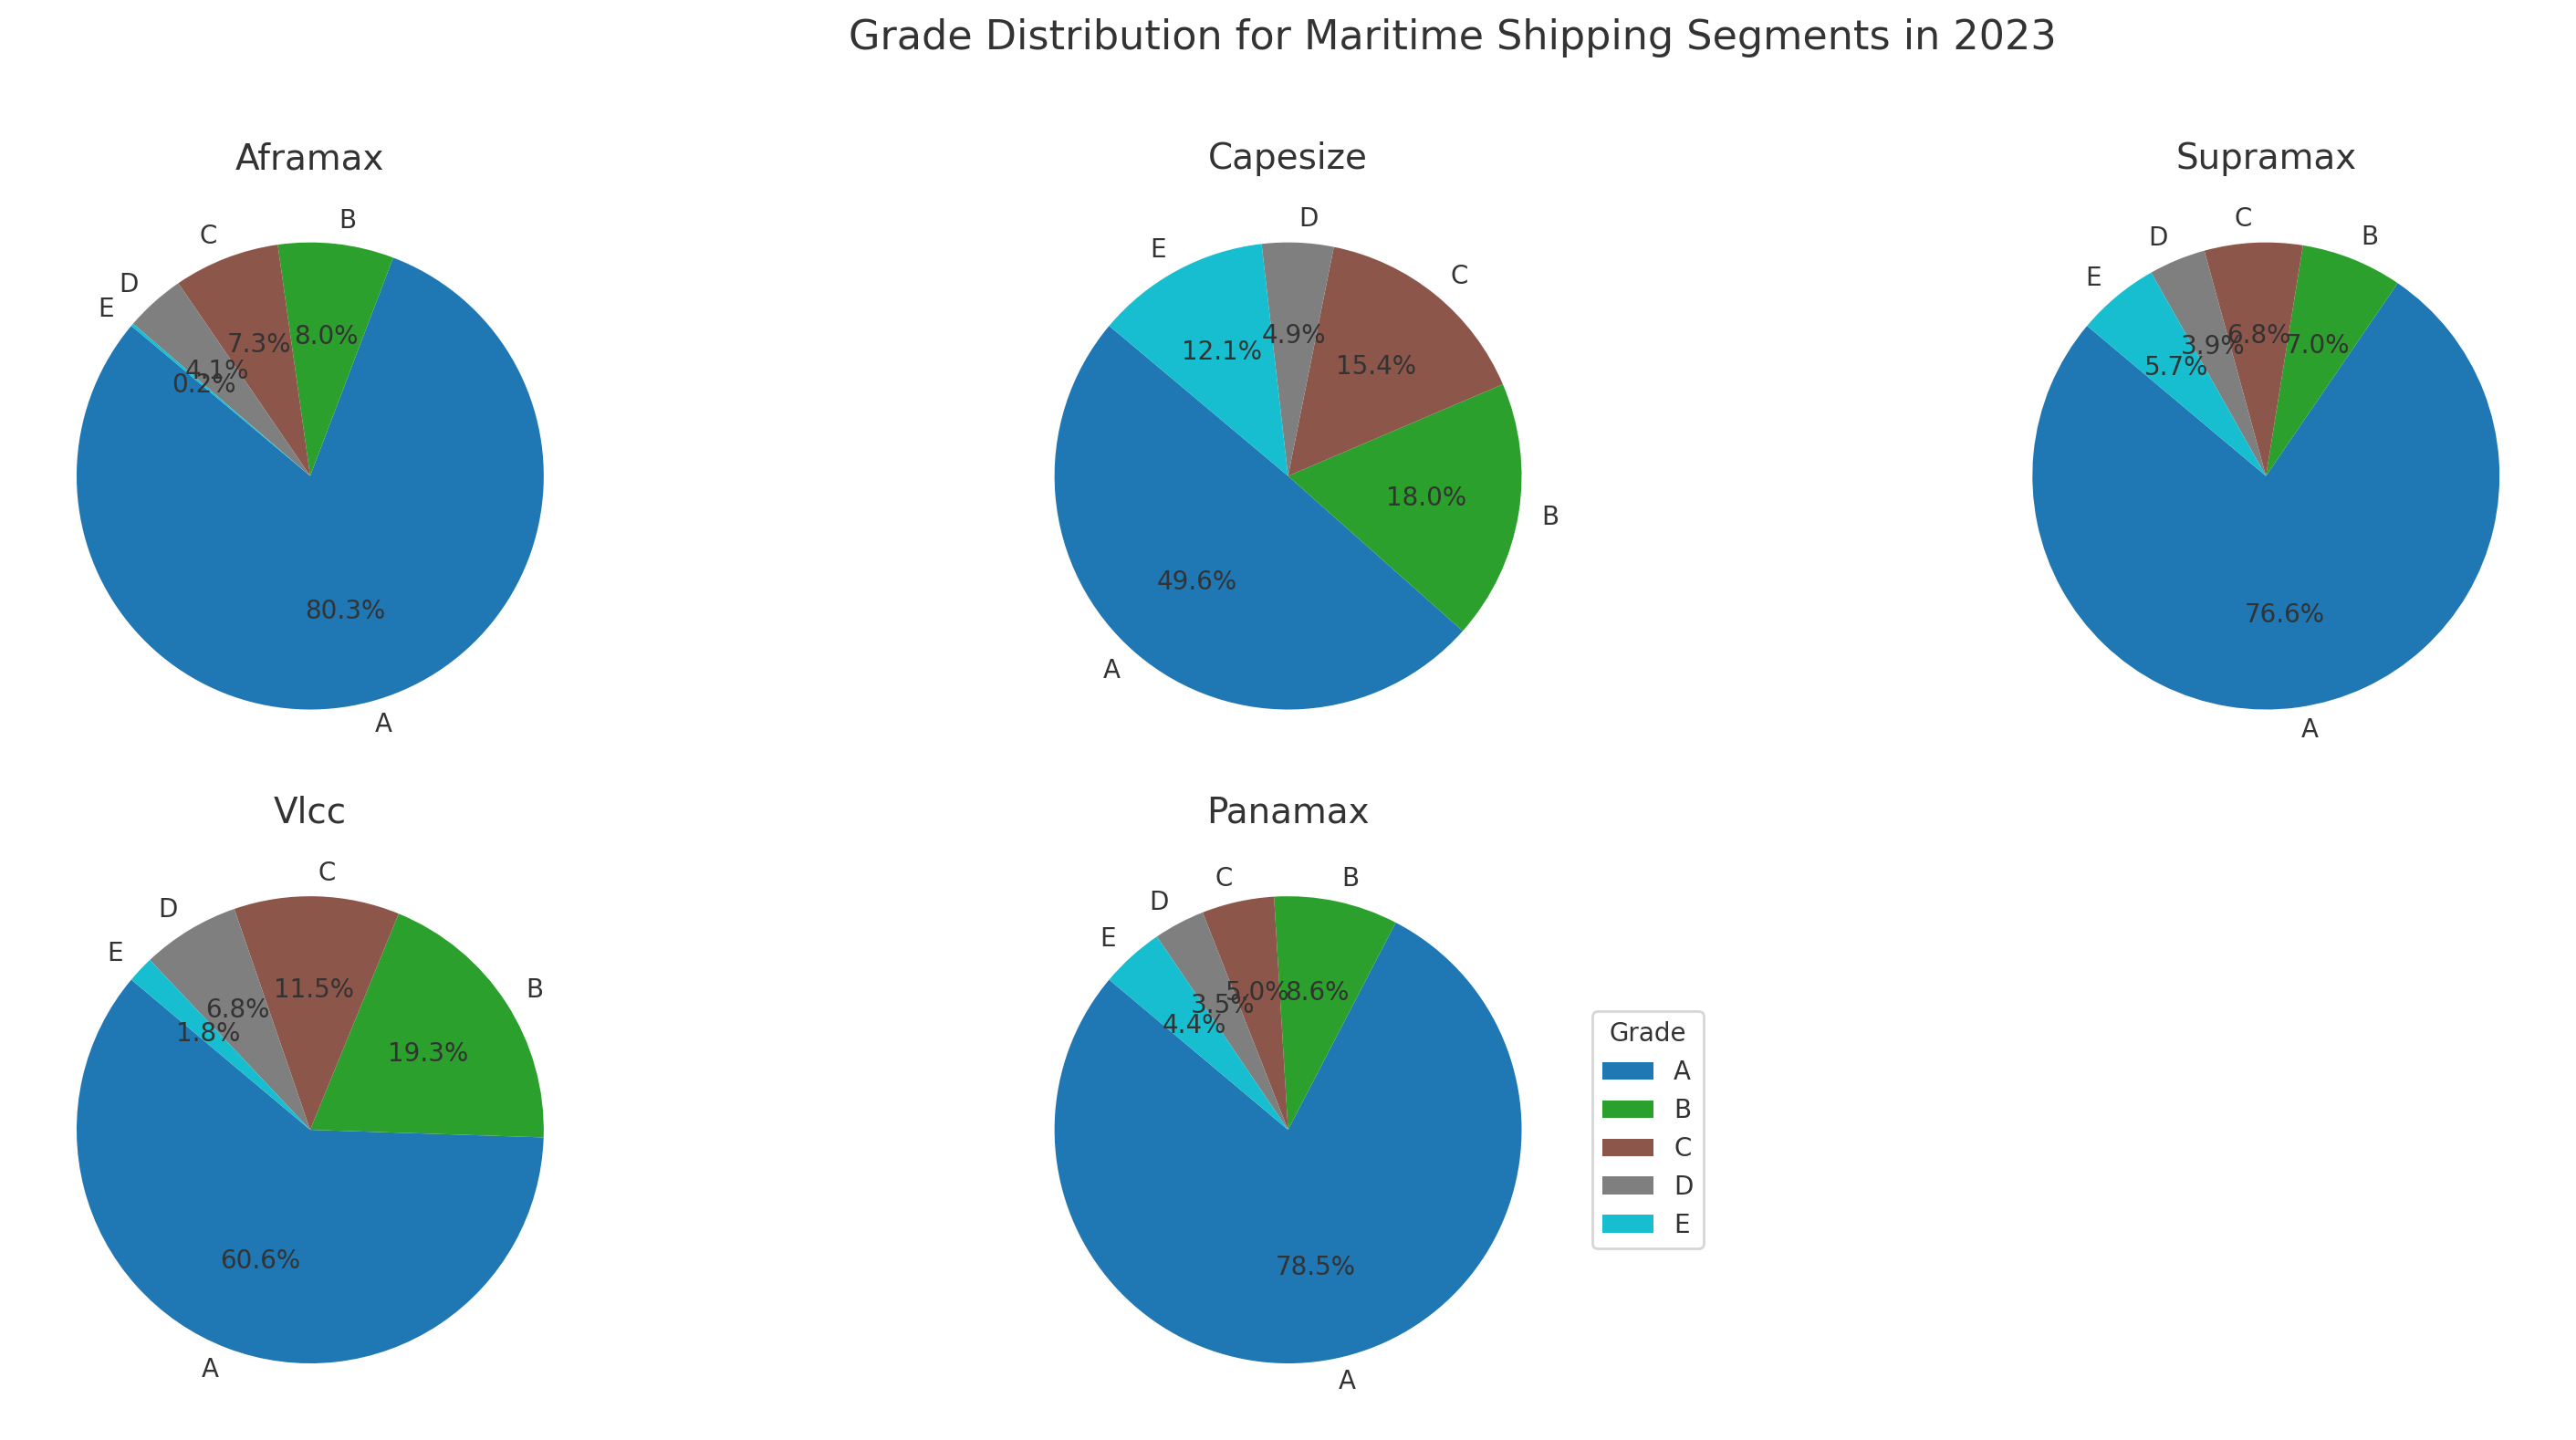
\includegraphics[width=0.8\textwidth]{images/grade_distribution.png}
    \caption{Grade Distribution}
    \label{grade_distribution}
\end{figure}


\begin{figure}[h]
    \centering
    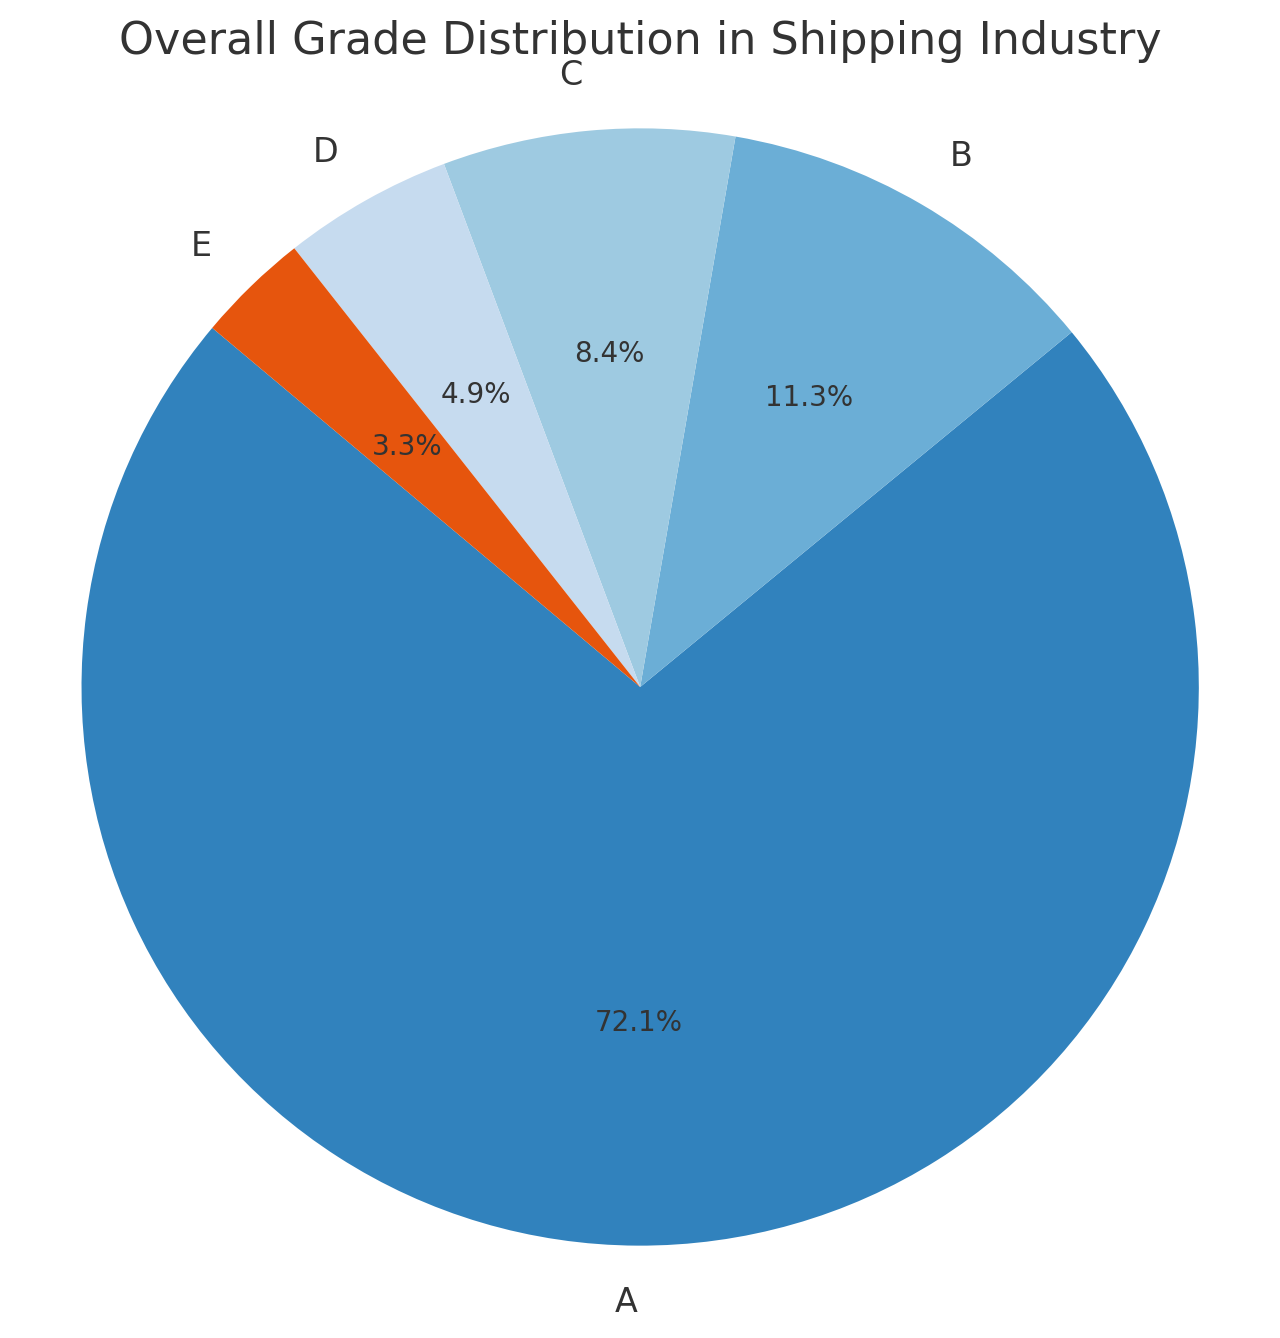
\includegraphics[width=0.8\textwidth]{images/combined_grade.png}
    \caption{Combined Grade}
    \label{combined_grade}
\end{figure}

he above Figure \ref{grade_distribution} depicts a plot of the CII grade distribution of the vessels based on segment. 
Figure \ref{combined_grade}, on the other hand, illustrates the grade distribution of all the vessels. 
It is evident that the Aframax segment has performed the best, with 80.3\% A-grade vessels and only 4.3\% of D and E-grade vessels.

However, an overarching trend emerges, wherein approximately 70\% of vessels obtained grade A or B, while only 8\% of vessels attained grade D or E.

\subsection{Grade Distribution Trend}

\begin{figure}[h]
    \centering
    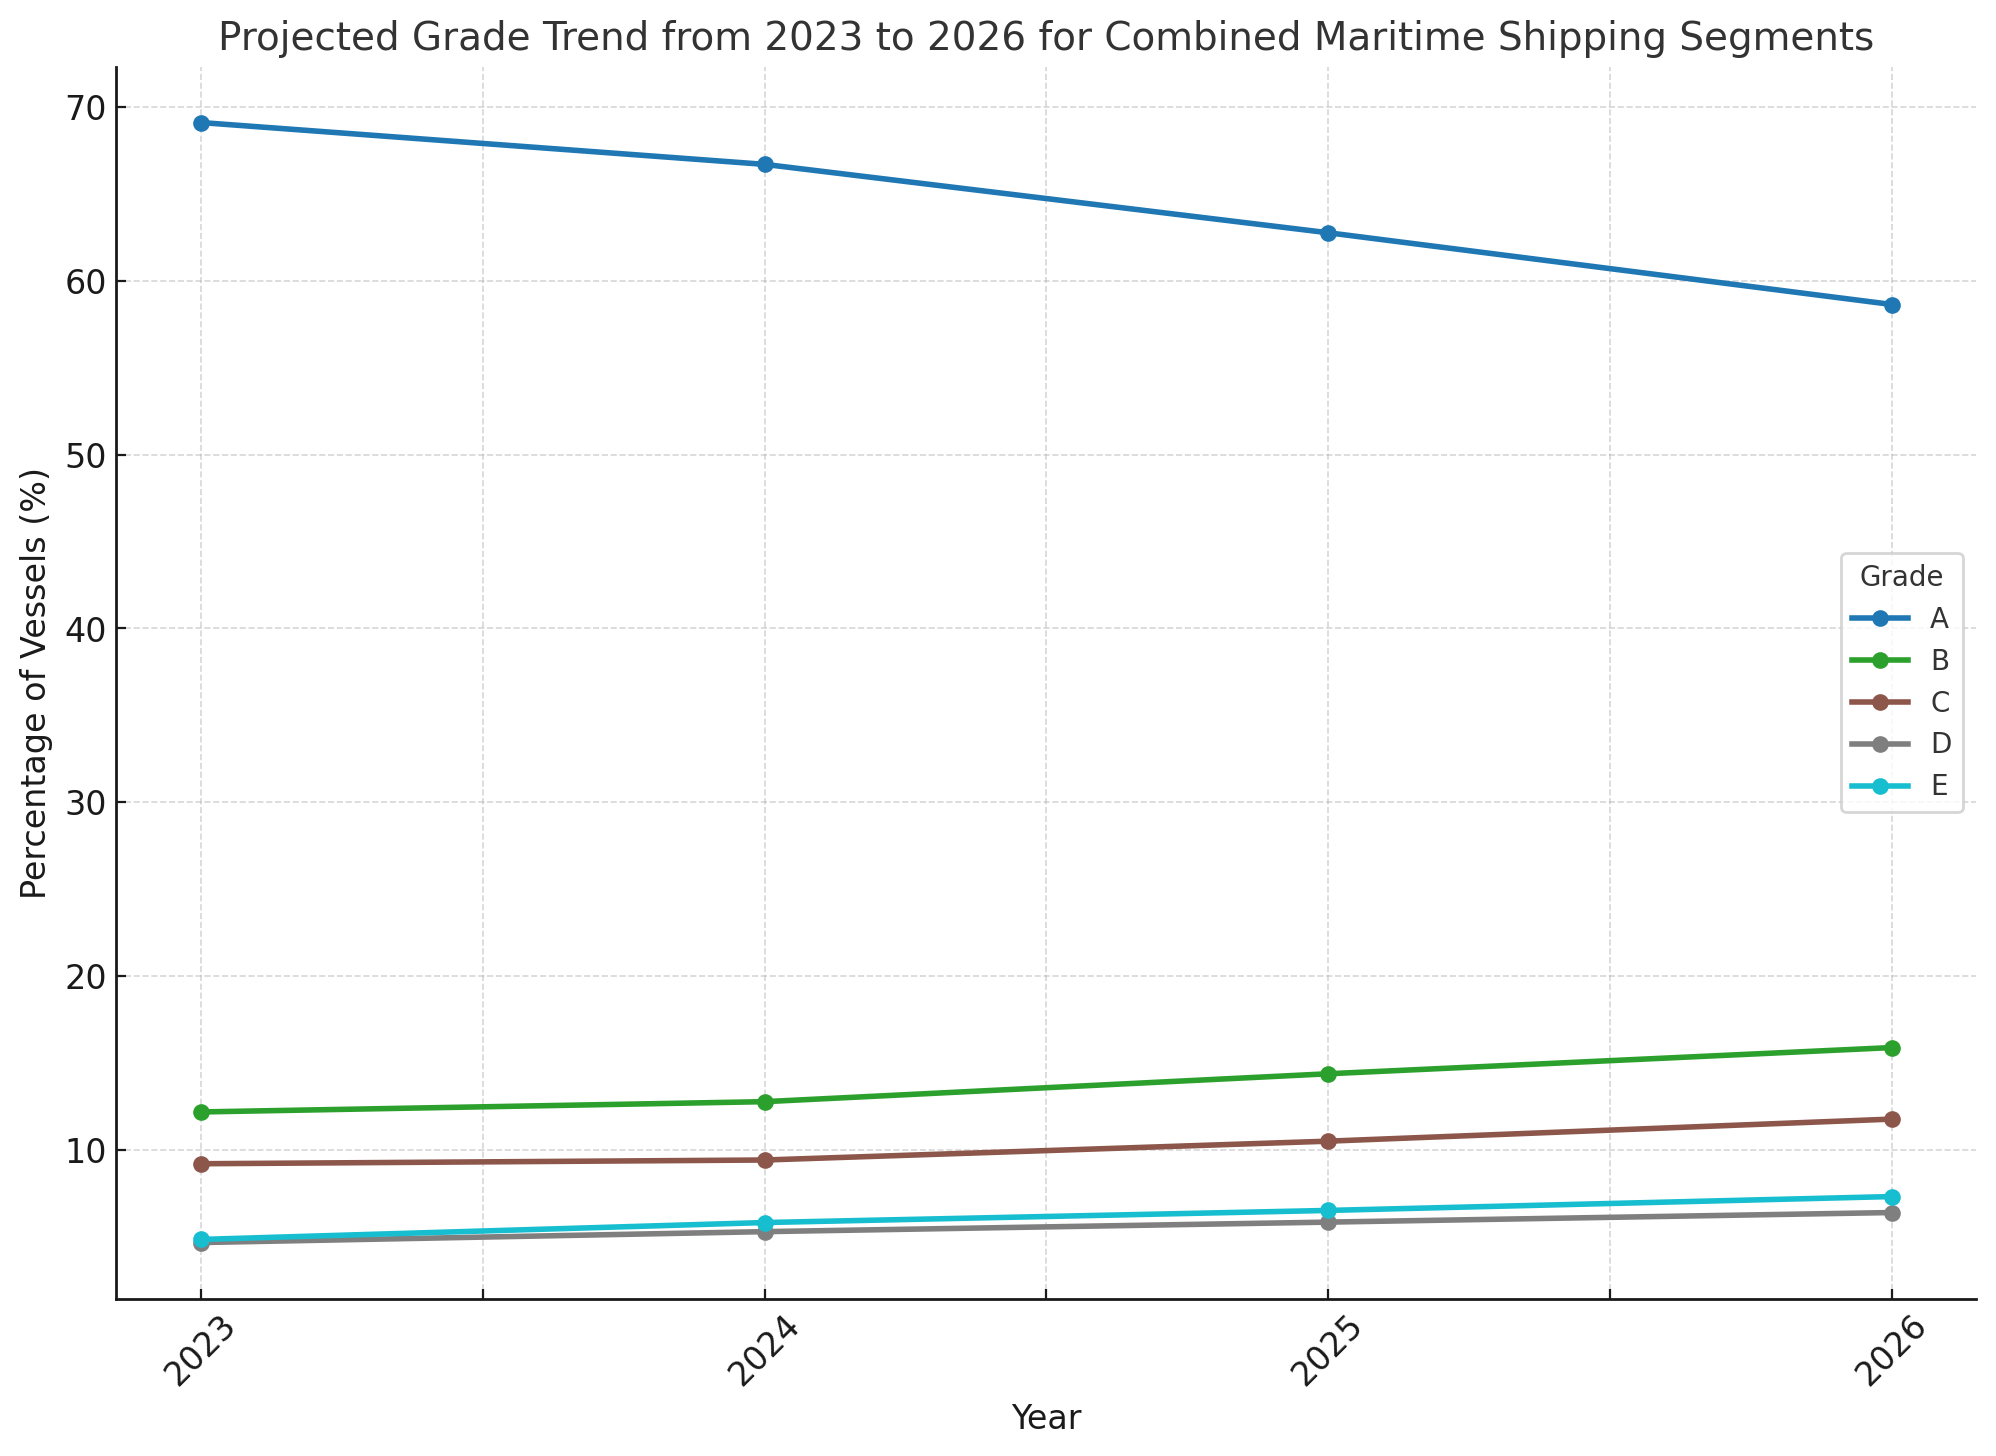
\includegraphics[width=0.8\textwidth]{images/grade_trend.png}
    \caption{Grade Distribution Trend}
    \label{grade_trend}
\end{figure}

In plot \ref{grade_trend} performace of vessels regards to grade over the years is highlighted.
It is apprant that the grades have worsened over the years if vessel follows similar trade flows.
Currently 70\% of vessels are in A or B grade, but in 2023 only about 50\% of vessels will be in A or B grade by 2026.

\newpage

\subsection{EEOI vs Grade}

\begin{figure}[h]
    \centering
    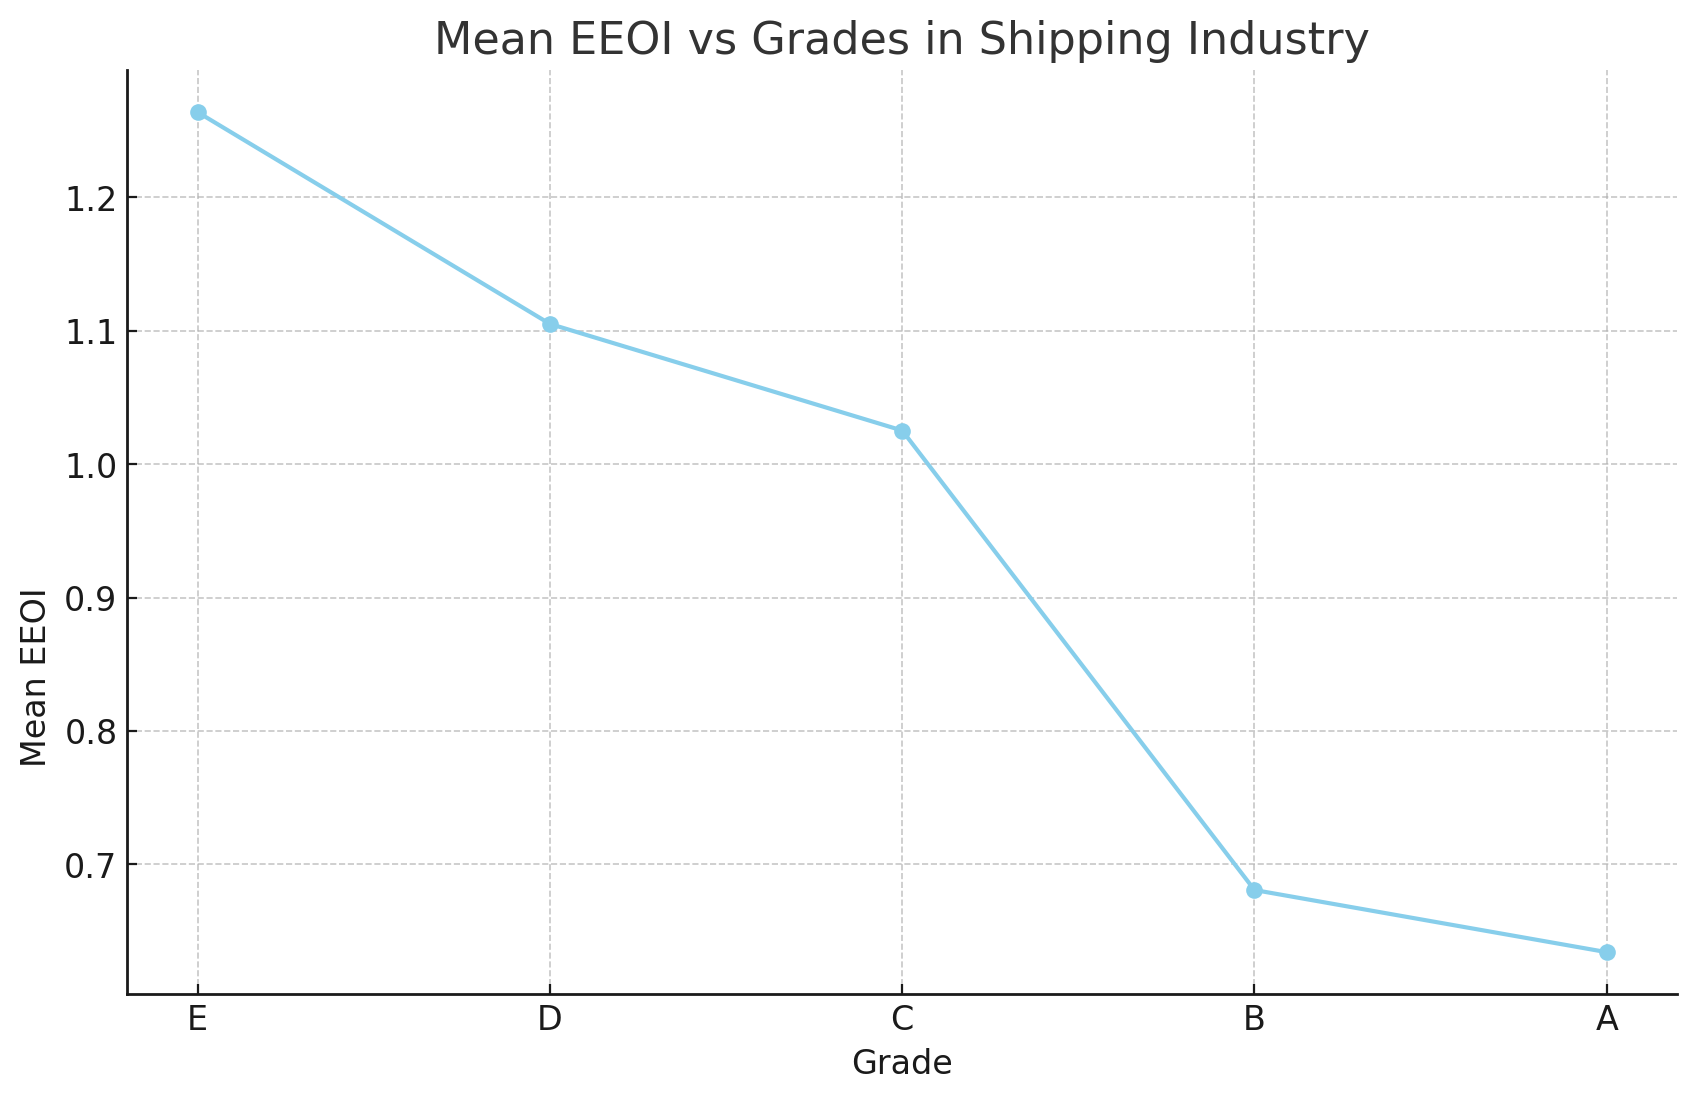
\includegraphics[width=0.8\textwidth]{images/eeoi_grade.png}
    \caption{Mean EEOI vs Grade}
    \label{eeoi_grade}
\end{figure}

The above Figure \ref{eeoi_grade} represnts realtionship between EEOI and grade.

Lower EEOI means vessels uses less fuel to achive same amount of work.
Based on the above plot it is clear that vessels with lower EEOI have better grade.
This signifies that vessels with lower EEOI are more fuel efficient and hence have better grade.


\begin{figure}[h]
    \centering
    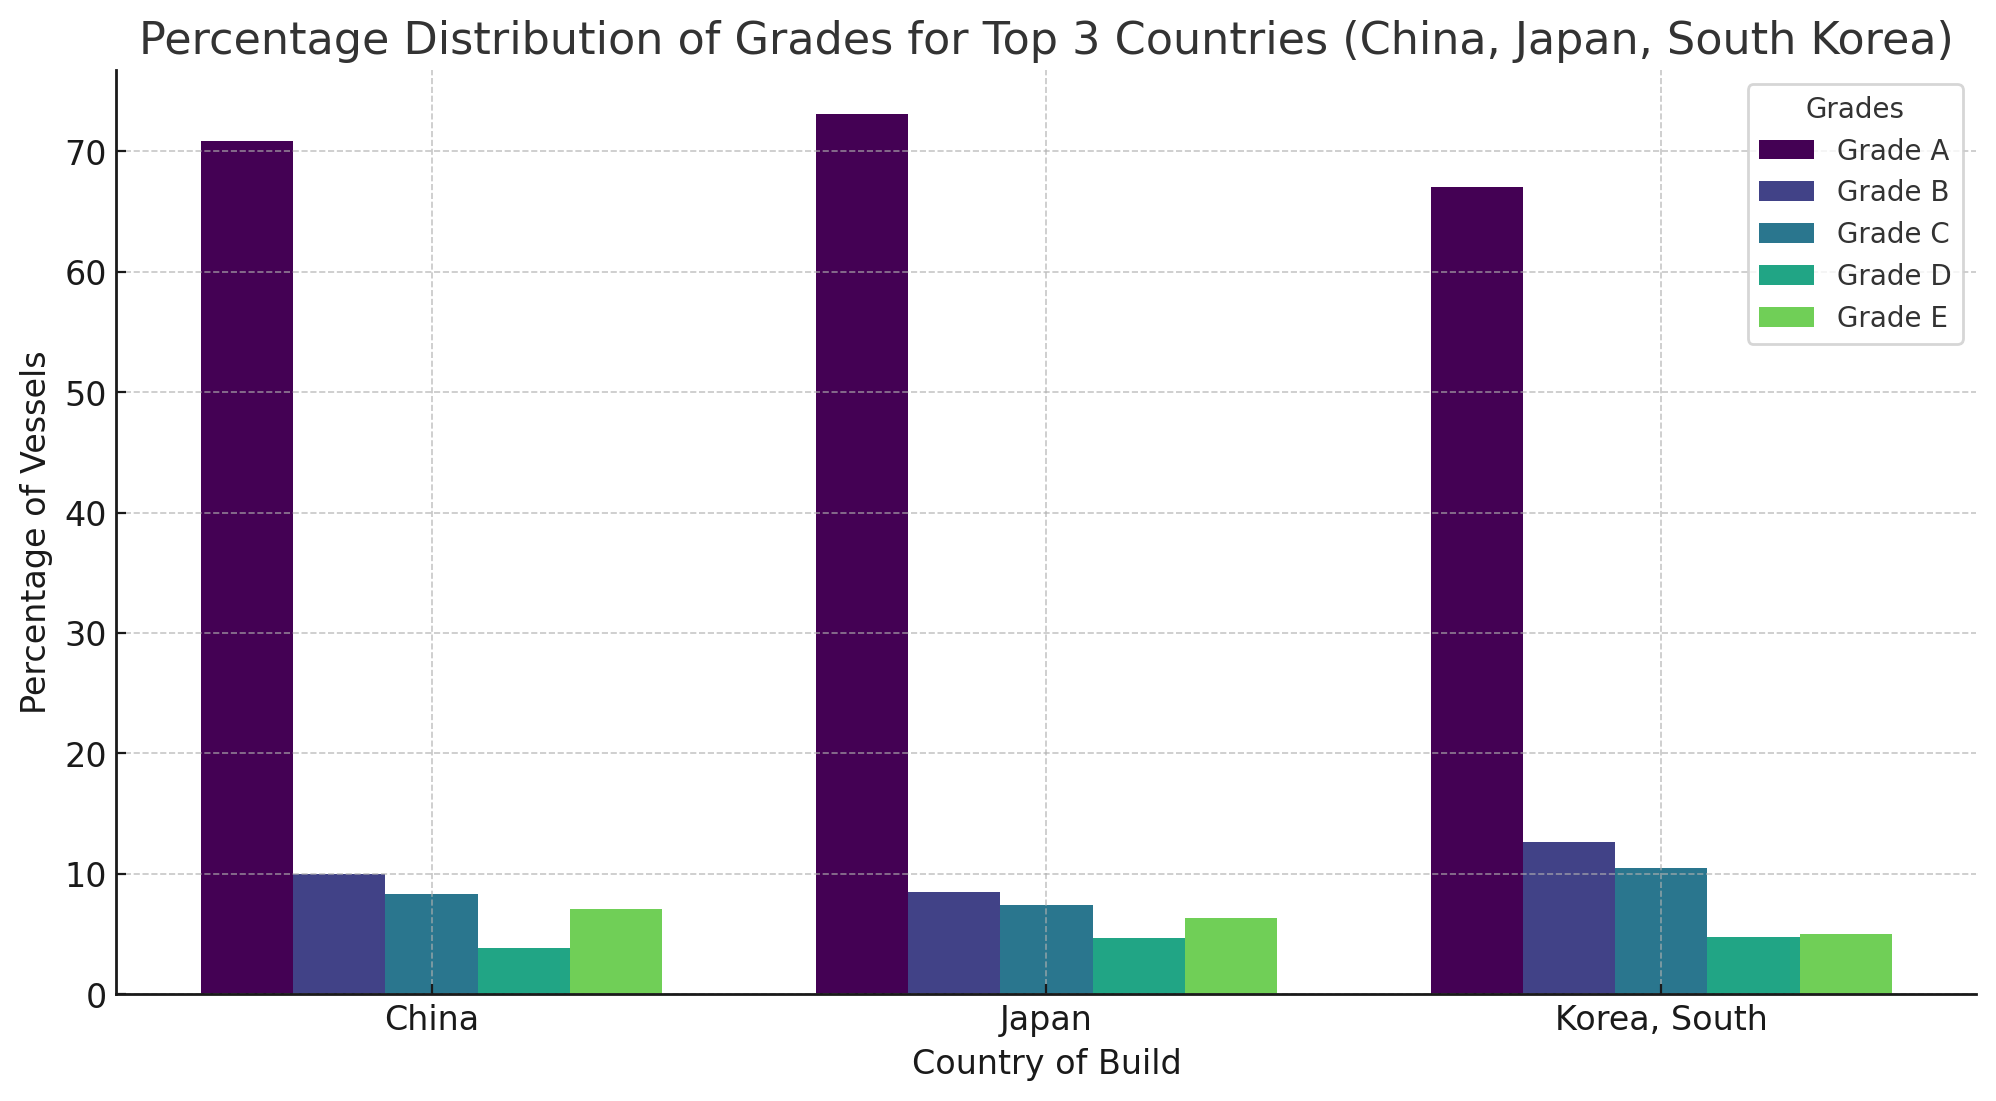
\includegraphics[width=0.8\textwidth]{images/grade_by_build_country.png}
    \caption{Grade By Build Country}
    \label{grade_by_build_country}
\end{figure}
